\documentclass[10pt, a4paper, titlepage]{article}

\usepackage{amsmath}
\usepackage{amssymb}
\usepackage{caption}
\usepackage{float}
\usepackage[portrait, margin=0.8cm]{geometry}
\usepackage{graphicx}
\graphicspath{{images/}}
\usepackage[none]{hyphenat}
\usepackage[utf8]{inputenc}
\usepackage{multicol}
\usepackage{physics}
\usepackage{sectsty}
\usepackage{subcaption}

%Removes equation label numbers
\makeatletter
\renewcommand\tagform@[1]{}
\makeatother

%Removes heading numbers of headers. Disable for numbers and to create table of contents.
\setcounter{secnumdepth}{0}

%Makes headers and footers empty: removes page numbers
\pagestyle{empty}

%Sets heading font sizes.
\sectionfont{\large}
\subsectionfont{\normalsize}

%Line between columns
%\setlength{\columnseprule}{0.4pt}

%\setlength{\parskip}{1em}

%Disables paragraph indents
\setlength{\parindent}{0em}

%Toggle column vertical alignment
\raggedcolumns

\title{12 Mathematical Methods Summarised Notes \\ (Unofficial)}
\author{}
\date{Last updated: July 2022}


\begin{document}
\maketitle
\begin{multicols*}{3}

\section{Differential Calculus}
	\subsection{Derivatives}
	The derivative of $y=f(x)$ is:
	\begin{align}
		\dv{y}{x} = f'(x) = \lim_{h\to 0}\frac{f(x+h)-f(x)}{h}
	\end{align}

	\dotfill
	\subsection{Simple Rules of Differentiation}
	\begin{flalign}
		&\quad \dv{x}\left[k\right] = 0&&\\
		&\quad \dv{x}\left[x^n\right] = nx^{n-1}&&\\
		&\quad \dv{x}\left[kf(x)\right] = k\dv{x}\left[f(x)\right] = kf'(x)&&\\
		&\quad \dv{x}\left[u(x)\pm v(x)\right] = u'(x)\pm v'(x)&&
	\end{flalign}

	\dotfill
	\subsection{Chain Rule}
	If $y=f(u(x))$, then
	\begin{align}
		\dv{y}{x} = \dv{y}{u}\times \dv{u}{x}
	\end{align}
	\begin{center}
		or
	\end{center}
	\begin{align}
		\dv{x}\left[f(g(x))\right] = f'(g(x))\cdot g'(x)
	\end{align}

	\dotfill
	\subsection{Product Rule}
	\begin{align}
		\dv{x}\left[u(x)v(x)\right] = u'(x)v(x)+u(x)v'(x)
	\end{align}

	\dotfill
	\subsection{Quotient Rule}
	\begin{align}
		\dv{x}\left[\frac{u(x)}{v(x)}\right] = \frac{u'(x)v(x)-u(x)v'(x)}{[v(x)]^2}
	\end{align}

	\dotfill
	\subsection{Exponential Functions}
	\begin{flalign}
		&\quad \dv{x}\left[e^x\right] = e^x&&\\
		&\quad \dv{x}\left[e^{f(x)}\right] = e^{f(x)}\times f'(x)&&
	\end{flalign}

	\dotfill
	\subsection{Natural Logarithm}
	\begin{align}
		\ln{x}=\log_{e}x
	\end{align}
	\underline{Natural Logarithm Laws:}
	\begin{align}
		&\ln{a}+\ln{b}=\ln{ab}&& &&\ln{e}=1&\\
		&\ln{a}-\ln{b}=\ln{\left(\frac{a}{b}\right)}&& &&\ln{e^x}=x&\\
		&\ln{(a^n)}=n\ln{a}&& &&e^{\ln{x}}=x&	
	\end{align}
	\underline{Graphing:}
	\begin{align}
		y=\ln{x}
	\end{align}
	\begin{itemize}
		\item asymptotic to the $y$-axis $(x=0)$
		\item passes through $(1,0)$
		\item domain: $x>0$, range: $y\in \mathbb{R}$
	\end{itemize}
	General Function:
	\begin{align}
		y=k\ln{(b(x-c))}
	\end{align}
	\begin{itemize}
		\item horizontal translation by $c$ units
		\item vertical translation by $k\ln{b}$ units
		\item vertical dilation scale factor $k$
	\end{itemize}

	\dotfill
	\subsection{Logarithmic Functions}
	\begin{flalign}
		&\quad \dv{x}\left[\ln{x}\right] = \frac{1}{x},\ x>0&&\\
		&\quad \dv{x}\left[\ln{f(x)}\right] = \frac{f'(x)}{f(x)}&&
	\end{flalign}

	\dotfill
	\subsection{Trigonometric Functions}
	\begin{flalign}
		&\quad \dv{x}\left[\sin{x}\right] = \cos{x}&&\\
		&\quad \dv{x}\left[\cos{x}\right] = -\sin{x}&&\\
		&\quad \dv{x}\left[\tan{x}\right] = \frac{1}{\cos^2{x}} = \sec^2{x}&&\\
		&\quad \dv{x}\left[\sin{[f(x)]}\right] = \cos{[f(x)]}f'(x)&&\\
		&\quad \dv{x}\left[\cos{[f(x)]}\right] = -\sin{[f(x)]}f'(x)&&\\
		&\quad \dv{x}\left[\tan{[f(x)]}\right] = \frac{f'(x)}{\cos^2{[f(x)]}}&&\\
		&\qquad \qquad = \sec^2{[f(x)]}f'(x) &&
	\end{flalign}


\hrulefill
\section{Applications of Derivatives}
	\subsection{Tangents}
	A line that touches a curve, matching the gradient of the curve at that point.\\
	To find the tangent to a curve $y=f(x)$ at $x=a$:
	\begin{enumerate}
		\item Find $\dv{y}{x}$ or $f'(x)$
		\item Find $y$-coordinate $y=f(a)$ and gradient $m=f'(a)$.
		\item Substitute values into $y=mx+c$ to find $c$.
	\end{enumerate}
	Or use general formula:
	\begin{align}
		y=f'(a)(x-a)+f(a)
	\end{align}

	\dotfill
	\subsection{Normals}
	A line that intersects a curve, perpendicular to the tangent at that point.\\
	For a normal to $y=f(x)$ at $x=a$, the gradient $m$ is the negative reciprocal of the tangent slope.
	\begin{align}
		m=-\frac{1}{f'(a)}
	\end{align}
	Normal general formula:
	\begin{align}
		y=-\frac{1}{f'(a)}(x-a)+f(a)
	\end{align}

	\dotfill
	\subsection{Stationary Points}
	The stationary point of a function is where the tangent is horizontal, and so, $f'(x)=0$.
	\begin{figure}[H]
		\centering
		\begin{subfigure}[b]{0.1\textwidth}
			\centering
			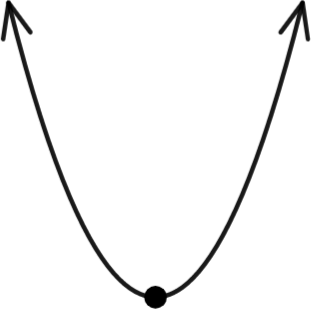
\includegraphics[width=0.8cm]{local_min.png}
			\caption*{Local\\min}
		\end{subfigure}
		\hfill
		\begin{subfigure}[b]{0.1\textwidth}
			\centering
			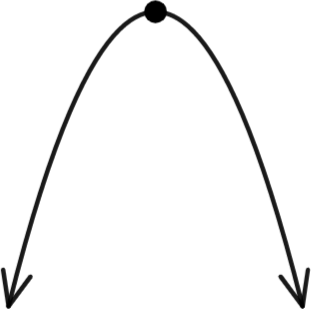
\includegraphics[width=0.8cm]{local_max.png}
			\caption*{Local\\max}
		\end{subfigure}
		\hfill
		\begin{subfigure}[b]{0.1\textwidth}
			\centering
			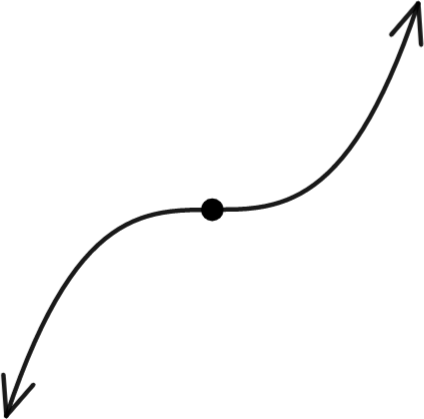
\includegraphics[width=0.8cm]{stat_inflection.png}
			\caption*{Stat inflection}
		\end{subfigure}
	\end{figure}
	Solve $f'(x)=0$ for $x$.\\
	Draw sign diagram of $f'(x)$\\
	Classify stationary points.\\

	\dotfill
	\subsection{Inflection Points}
	The inflection point on a curve is where the shape of the curve changes, when $f''(x)=0$.
	\begin{figure}[H]
		\centering
		\begin{subfigure}[b]{0.1\textwidth}
			\centering
			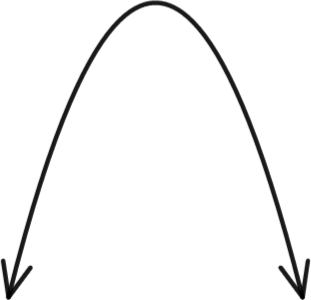
\includegraphics[width=0.8cm]{concave.png}
			\caption*{Concave,\\$f''(x)<0$}
		\end{subfigure}
		\hfill
		\begin{subfigure}[b]{0.1\textwidth}
			\centering
			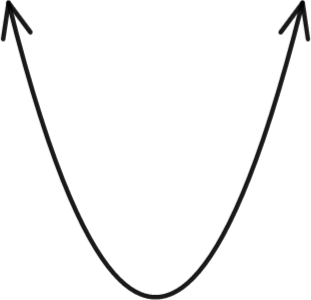
\includegraphics[width=0.8cm]{convex.png}
			\caption*{Convex,\\$f''(x)>0$}
		\end{subfigure}
		\\
		\centering
		\begin{subfigure}[b]{0.1\textwidth}
			\centering
			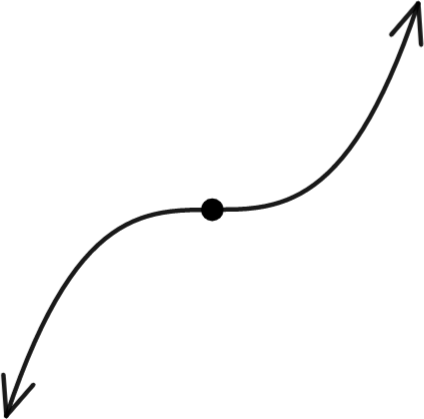
\includegraphics[width=0.8cm]{stat_inflection.png}
			\caption*{Stat\\inflection}
		\end{subfigure}
		\hfill
		\begin{subfigure}[b]{0.1\textwidth}
			\centering
			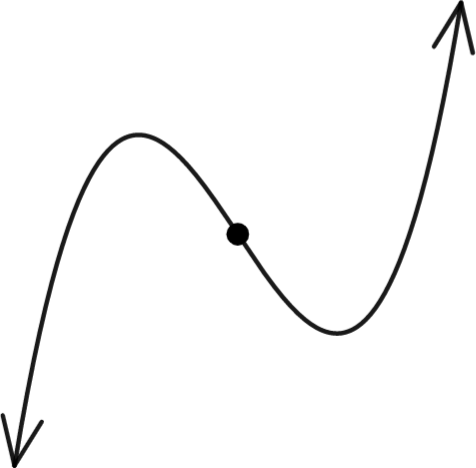
\includegraphics[width=0.8cm]{non_stat_inflection.png}
			\caption*{Non-stat\\inflection}
		\end{subfigure}
	\end{figure}
	Solve $f''(x)=0$ for $x$.\\
	Classify inflection points:\\
	If $f'(x)=0$, stationary.\\
	If $f'(x)\neq 0$, non-stationary.\\

	\dotfill
	\subsection{Sketching Graphs of Derivatives}
	\underline{Sketching $y=f'(x)$ from $y=f(x)$:}
	\begin{enumerate}
		\item Stat point $f(x)$ $\rightarrow$ zero of $f'(x)$
		\item If $f(x)$ increasing, $f'(x)$ positive
		\item If $f(x)$ decreasing, $f'(x)$ negative
		\item If $f(x)$ convex, $f'(x)$ increasing
		\item If $f(x)$ concave, $f'(x)$ decreasing
		\item Infl point $f(x)$ $\rightarrow$ stat point $f'(x)$
		\item Asymp $f(x)$ $\rightarrow$ asymp $f'(x)$
	\end{enumerate}
	Reverse to sketch $f(x)$ from $f'(x)$.\\\\
	\underline{Sketching $y=f''(x)$ from $y=f(x)$:}
	\begin{enumerate}
		\item Infl point $f(x)$ $\rightarrow$ zero of $f''(x)$
		\item If $f(x)$ convex, $f''(x)$ positive
		\item If $f(x)$ concave, $f''(x)$ negative
		\item Asymp $f(x)$ $\rightarrow$ asymp $f''(x)$
	\end{enumerate}
	Reverse to sketch $f'(x)$ from $f''(x)$.\\

	\dotfill
	\subsection{Kinematics}
	Describing the motion of moving objects.
	\begin{flalign}
		&\text{Displacement:}\quad s(t)&&\\
		&\text{Velocity:}\quad v(t)=s'(t)&&\\
		&\text{Acceleration:}\quad a(t)=v'(t)=s''(t)&&
	\end{flalign}
	\underline{Motion Diagrams:}
	\begin{itemize}
		\item Start position
		\item Time and position of direction change
		\item End position
	\end{itemize}
	\begin{center}
		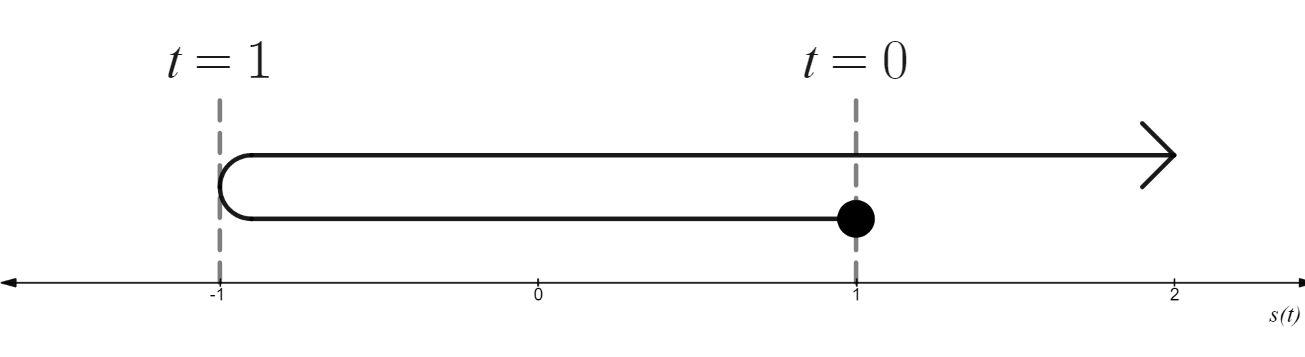
\includegraphics[width=0.9\linewidth]{motion_diagram.png}\\
	\end{center}
	Speed increasing when $v(t)$ and $a(t)$ have the same sign. Decreasing when it is a different sign.\\

	\dotfill
	\subsection{Optimisation}
	Optimisation is finding the max/min value of a function, often called the optimal solution.
	\begin{enumerate}
		\item Draw a diagram.
		\item Construct a formula with the value to be optimised as the subject.
		\item Find the first derivative and its zeros.
		\item Use a sign diagram to determine the nature of stationary points.
		\item Identify the optimal solution.
		\item Write the answer as a sentence.
	\end{enumerate}


\hrulefill
\section{Integral Calculus}
	\subsection{Antidifferentiation}
	The reverse process of differentiation.\\
	$F(x)$ is a function where $F'(x)=f(x)$.
	\begin{itemize}
		\item The derivative of $F(x)$ is $f(x)$
		\item The antiderivative of $f(x)$ is $F(x)$
	\end{itemize}

	\dotfill
	\subsection{Indefinite Integrals}
	\begin{flalign}
		&\quad \int k\,\dd{x} = kx+c&&\\
		&\quad \int x^n\,\dd{x} = \frac{1}{n+1}x^{n+1}+c,\ n\neq -1&&\\
		&\quad \int e^x\,\dd{x} = e^x+c&&\\
		&\quad \int \frac{1}{x}\,\dd{x} = \ln|x|+c&&\\
		&\quad \int \cos{x}\,\dd{x} = \sin{x}+c&&\\
		&\quad \int \sin{x}\,\dd{x} = -\cos{x}+c&&
	\end{flalign}

	\dotfill
	\subsection{Integrating $f(ax+b)$}
	\begin{flalign}
		&\quad \int (ax+b)^n\,\dd{x} = \frac{(ax+b)^{n+1}}{a(n+1)}+c,&&\\
		&\quad \qquad n\neq -1&&\\
		&\quad \int e^{ax+b}\,\dd{x} = \frac{1}{a}e^{ax+b}+c&&\\
		&\quad \int \frac{1}{ax+b}\,\dd{x} = \frac{1}{a}\ln|ax+b|+c&&\\
		&\quad \int \cos(ax+b)\,\dd{x}&&\\
		&\quad \qquad \frac{1}{a}\sin(ax+b)+c&&\\
		&\quad \int \sin(ax+b)\,\dd{x}&&\\
		&\quad \qquad = -\frac{1}{a}\cos(ax+b)+c&&\\
	\end{flalign}

	\dotfill
	\subsection{Definite Integrals}
	If $F(x$) is the antiderivative of $f(x)$ where $f(x)$ is continuous over $a\leq x\leq b$, the definite integral is:
	\begin{align}
		\int_{a}^{b}f(x)\,\dd{x} = F(b)-F(a)
	\end{align}

	\dotfill
	\subsection{Properties of Definite Integrals}
	\begin{flalign}
		&\quad \int_{a}^{a}f(x)\,\dd{x} = 0&&\\
		&\quad \int_{a}^{b}k\,\dd{x} = k(b-a)&&\\
		&\quad \int_{a}^{b}f(x)\,\dd{x} = -\int_{b}^{a}f(x)\,\dd{x}&&\\
		&\quad \int_{a}^{b}kf(x)\,\dd{x} = k\int_{a}^{b}f(x)\,\dd{x}&&\\
		&\quad \int_{a}^{b}f(x)\,\dd{x} +\int_{b}^{c}f(x)\,\dd{x}&&\\
		&\quad \qquad = \int_{a}^{c}f(x)\,\dd{x}&&\\
		&\quad \int_{a}^{b}\left[f(x)\pm g(x)\right]\,\dd{x}&&\\
		&\quad \qquad = \int_{a}^{b}f(x)\,\dd{x} \pm \int_{a}^{b}g(x)\,\dd{x}&&
	\end{flalign}

	\dotfill
	\subsection{Underestimating and \\Overestimating}
	\underline{Underestimating:}\\
	\begin{center}
		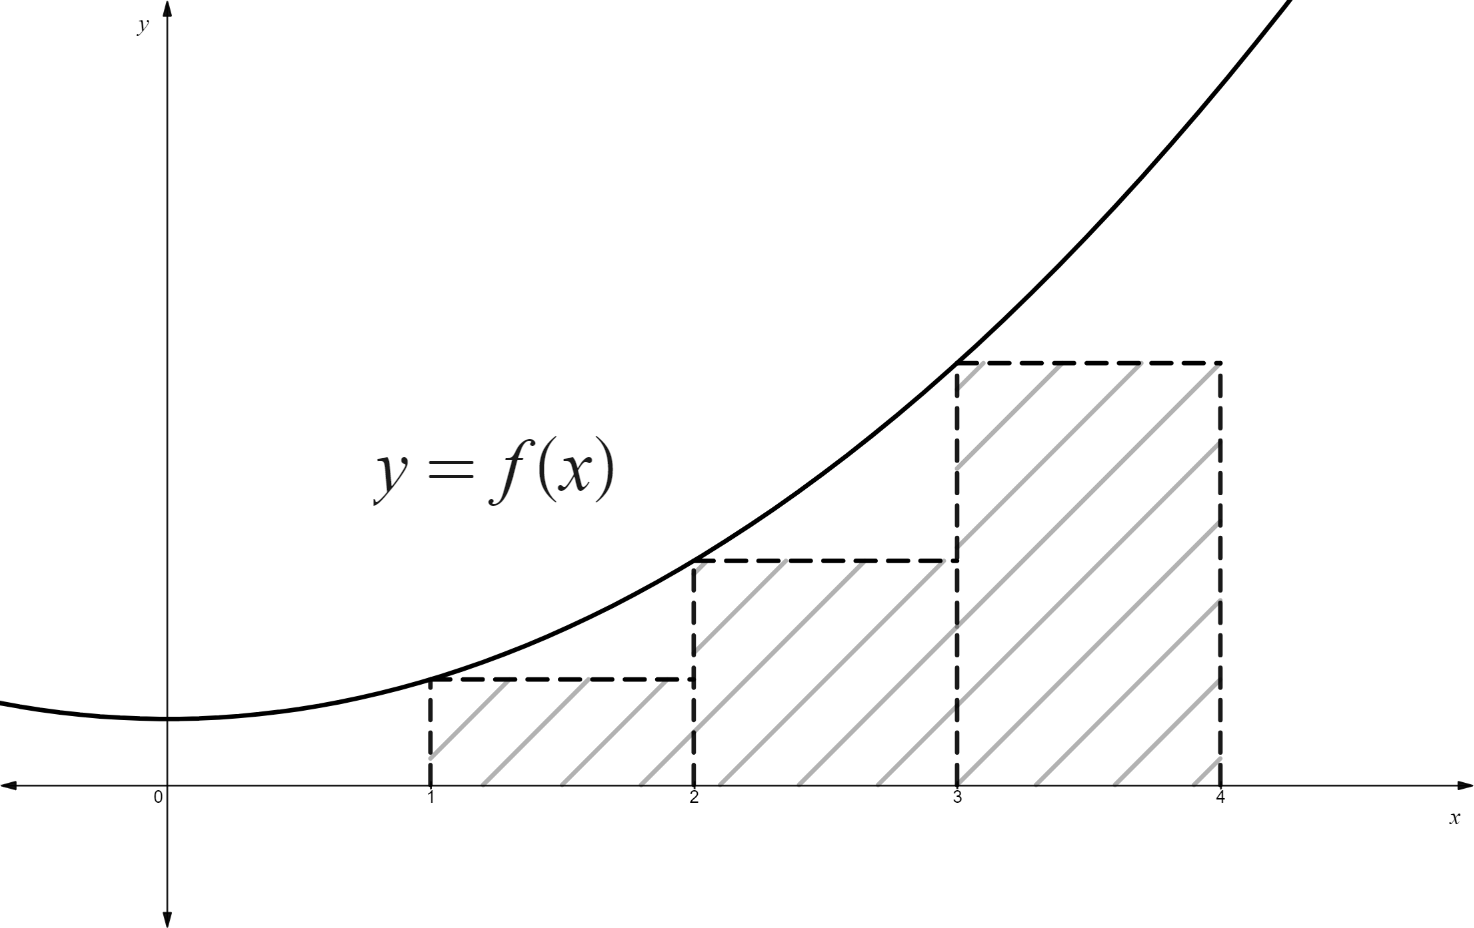
\includegraphics[width=0.9\linewidth]{underestimate.png}\\
	\end{center}
	\begin{align}
		A_L=1\times f(1)+1\times f(2)+1\times f(3)
	\end{align}
	\underline{Overestimating:}\\
	\begin{center}
		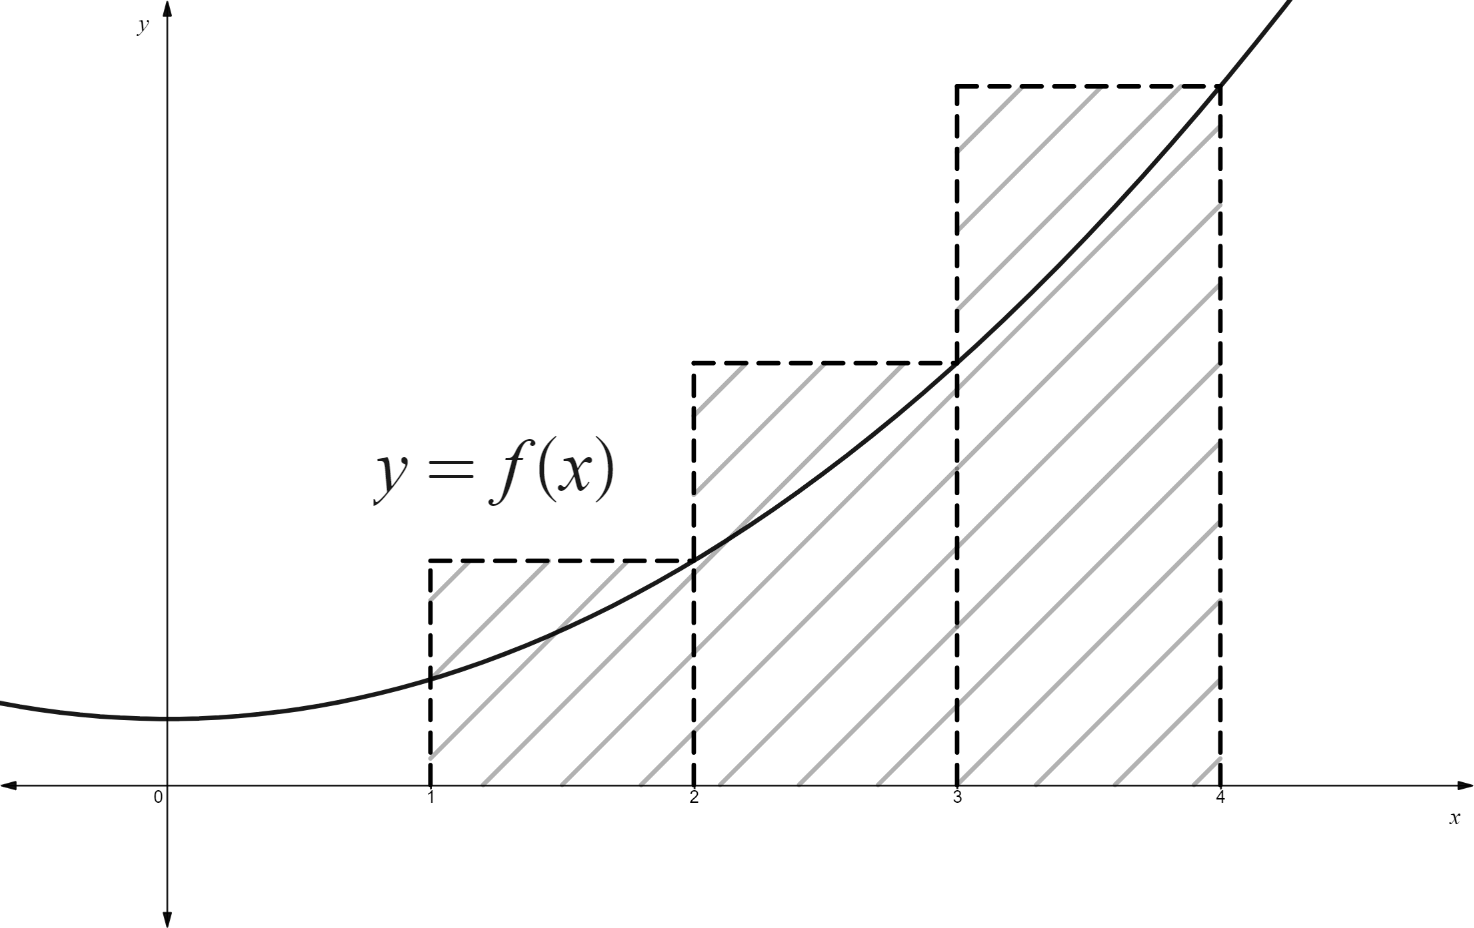
\includegraphics[width=0.9\linewidth]{overestimate.png}\\
	\end{center}
	\begin{align}
		A_U&=1\times f(2)+1\times f(3)+1\times f(4)\\
		&\therefore A_L\leq A\leq A_U
	\end{align}
	If the graph is convex, an underestimate is more accurate.\\
	If the graph is concave, an overestimate is more accurate.\\

	\dotfill
	\subsection{Area Under a Curve}
	If $f(x)$ is positive and continuous for $a\leq x\leq b$, the area bound by $y=f(x)$, the $x$-axis, $x=a$ and $x=b$ is:
	\begin{align}
		A=\int_{a}^{b}f(x)\,\dd{x}\qquad \text{or}\qquad A=\int_{a}^{b}y\,\dd{x}
	\end{align}
	\begin{center}
		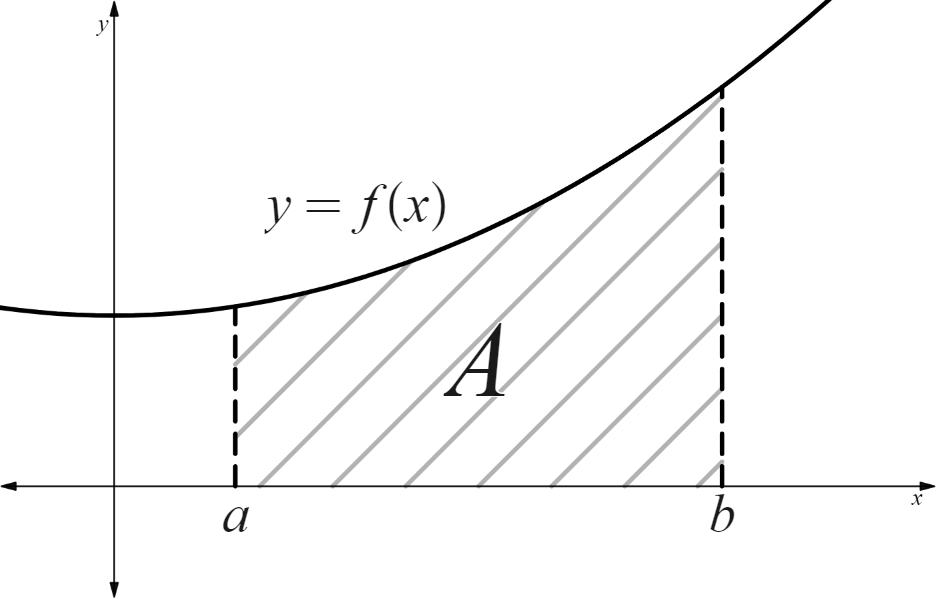
\includegraphics[width=0.9\linewidth]{area_under_a_curve.png}\\
	\end{center}

	\dotfill
	\subsection{Area Between Two Curves}
	Upper function: $f(x)$ or $y_U$\\
	Lower function: $g(x)$ or $y_L$
	\begin{align}
		A=\int_{a}^{b}\left[f(x)-g(x)\right]\,\dd{x}
	\end{align}
	\begin{center}
		or
	\end{center}
	\begin{align}
		A=\int_{a}^{b}\left[y_U-y_L\right]\,\dd{x}
	\end{align}
	\begin{center}
		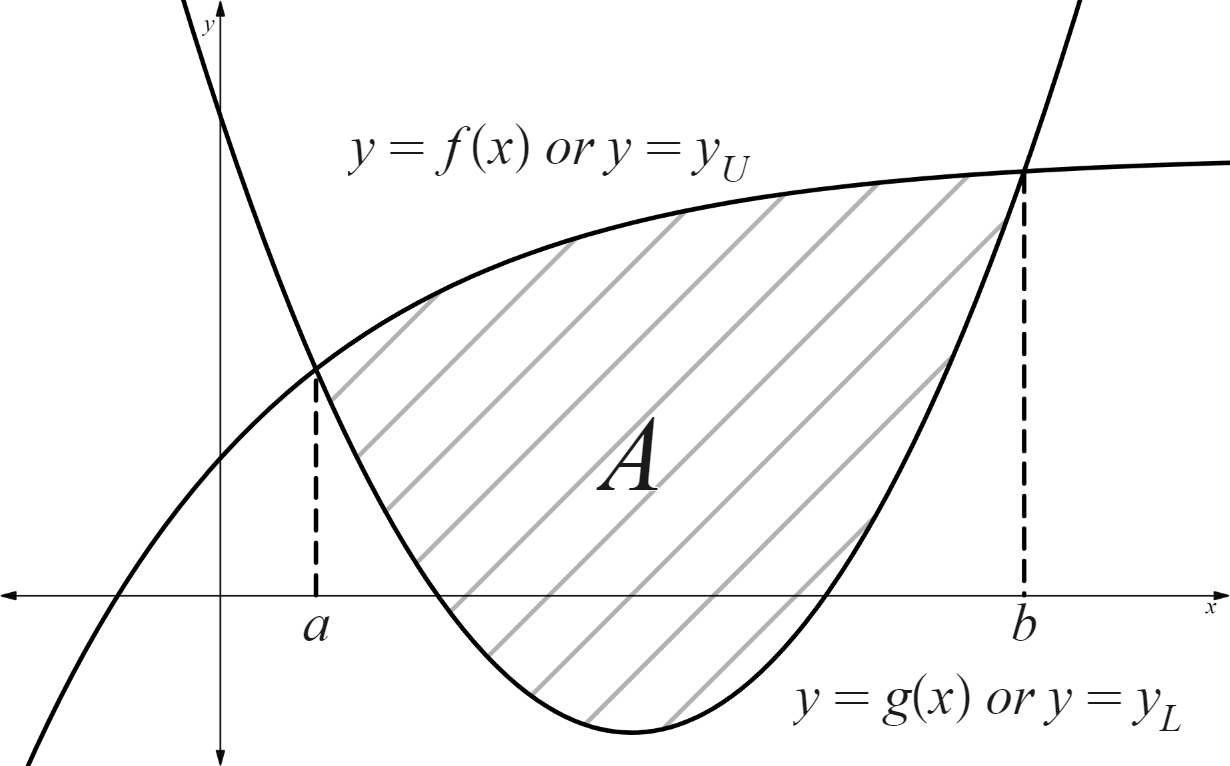
\includegraphics[width=0.9\linewidth]{area_between_two_curves.png}\\
	\end{center}

	\dotfill
	\subsection{Kinematics}
	For a velocity time function $v(t)$ where $v(t)\geq 0$ on the interval $t_1\leq t\leq t_2$
	\begin{align}
		\text{distance travelled} = \int_{t_1}^{t_2}|v(t)|\,\dd t
	\end{align}
	Displacement function:
	\begin{align}
		s(t) = \int_{t_1}^{t_2} v(t)\,\dd t
	\end{align}


\hrulefill
\section{Statistics}
	\subsection{Discrete Random Variables}
	Random variable $X$ with distinct possible values ${x_1, x_2, x_3,\dots , x_n}$ and corresponding probabilities $\{p_1, p_2, p_3,\dots , p_n\}$
	\begin{flalign}
		&\quad P(X=x_i)=p_i&&\\
		&\quad 0\leq p_i\leq 1\ \forall \ i=1,2,3,\dots ,n&&\\
		&\quad \sum_{i=1}^{n}p_i=p_1+p_2+p_3+\dots +p_n=1&&
	\end{flalign}

	\dotfill
	\subsection{Mean/Expected Value}
	The mean/expected value of discrete random variable $X$ is:
	\begin{align}
		E(X)&=\mu =\sum_{i=1}^{n}x_ip_i\\
		&=x_1p_1+x_2p_2+\dots +x_np_n
	\end{align}

	\dotfill
	\subsection{Fair Games}
	If $X$ represents the gain of a player from each game, the game is fair if $E(X)=0$.

	\dotfill
	\subsection{Variance and Standard Deviation}
	Variance: Average squared deviation from the mean.
	\begin{align}
		\text{Var}(X)=\sigma ^2=\sum (x_i-\mu)^2p_i
	\end{align}
	\begin{center}
		or
	\end{center}
	\begin{align}
		\text{Var}(X)=\sigma ^2=\sum x_i^2p_i-\mu ^2
	\end{align}
	Standard Deviation: Average deviations from the mean.
	\begin{align}
		\sigma =\sqrt{\sum (x_i-\mu)^2p_i}
	\end{align}
	\begin{center}
		or
	\end{center}
	\begin{align}
		\sigma =\sqrt{\sum x_i^2p_i-\mu ^2}
	\end{align}

	\dotfill
	\subsection{Bernoulli Distribution}
	A Bernoulli random variable $X$ can only take two values:
	\begin{itemize}
		\item $X=1$ is ``success"
		\item $X=0$ is ``failure"
		\item Only one trial is conducted
	\end{itemize}
	\begin{flalign}
		&\text{Mean:}\quad E(X)=\mu = p&&\\
		&\text{Variance:}\quad \text{Var}(X)=\sigma ^2=p(1-p)&&\\
		&\text{Standard Deviation:}\quad \sigma =\sqrt{p(1-p)}&&\\
	\end{flalign}

	\dotfill
	\subsection{Binomial Distribution}
	If there are $n$ independent trials with probability $p$ of success, the probability there are $k$ successes is:
	\begin{align}
		P(X=k)=\binom{n}{k}p^k(1-p)^{n-k}\\
		\text{where}\ k=1,2,3,\dots ,n
	\end{align}
	Binomial random variable $X$ is denoted:
	\begin{align}
		X\sim B(n,p)
	\end{align}
	\begin{flalign}
		&\text{Mean:}\quad E(X)=\mu = np&&\\
		&\text{Variance:}\quad \text{Var}(X)=\sigma ^2=np(1-p)&&\\
		&\text{Standard Deviation:}\quad \sigma =\sqrt{np(1-p)}&&\\
	\end{flalign}

	\dotfill
	\subsection{Probability Density Functions}
	For a continuous random variable $X$ on domain $a\leq x\leq b$ has probability density function $f(x)$ such that:
	\begin{align}
		P(a\leq x\leq b)=\int_{a}^{b}f(x)\,\dd{x}
	\end{align}
	\begin{flalign}
		&\quad f(x)\geq 0\ \forall \ a\leq X\leq b&&\\
		&\quad \int_{a}^{b}f(x)\,\dd{x} = 1&&
	\end{flalign}
	Mode: Value of $x$ which maximises $f(x)$ on $a\leq x\leq b$.\\
	Median: Value of $m$ such that:
	\begin{align}
		\int_{a}^{m}f(x)\,\dd{x} = \frac{1}{2}
	\end{align}
	\begin{flalign}
		&\text{Mean:}&&\\
		&\quad E(X)=\mu = \int_{a}^{b}xf(x)\,\dd{x}&&\\
		&\text{Variance:}\\
		&\quad \text{Var}(X)=\sigma ^2=\int_{a}^{b}x^2f(x)\,\dd{x}-\mu ^2&&\\
		&\text{or}&&\\
		&\quad \text{Var}(X)=\sigma ^2=\int_{a}^{b}(x-\mu)^2f(x)\,\dd{x}&&\\
		&\text{Standard Deviation:}&&\\
		&\quad \sigma =\sqrt{\int_{a}^{b}x^2f(x)\,\dd{x}-\mu ^2}&&\\
		&\text{or}&&\\
		&\quad \sigma =\sqrt{\int_{a}^{b}(x-\mu)^2f(x)\,\dd{x}}&&
	\end{flalign}

	\dotfill
	\subsection{Normal Distribution}
	\begin{center}
		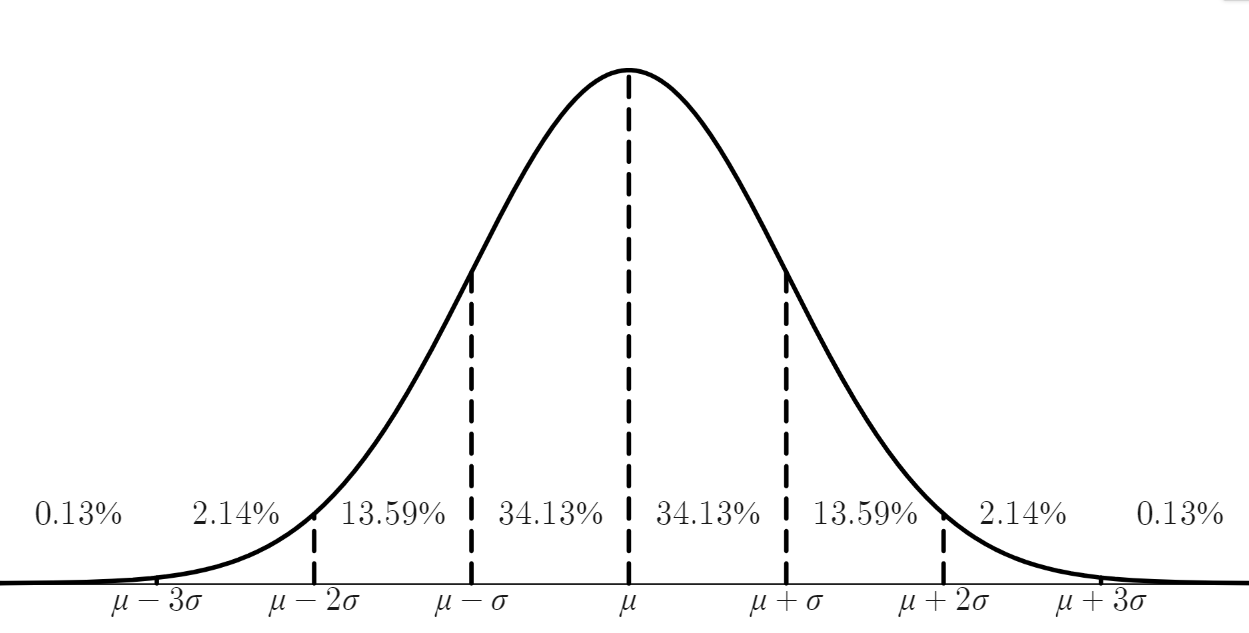
\includegraphics[width=0.9\linewidth]{normal_distribution.png}\\
	\end{center}
	\begin{align}
		f(x)=\frac{1}{\sigma \sqrt{2\pi}}e^{-\frac{1}{2}\left(\frac{x-\mu}{\sigma}\right)^2}\\
		\text{for }-\infty <x<\infty
	\end{align}
	\begin{itemize}
		\item Symmetric about the mean
		\item Bell shaped curve
		\item Asymptotic to the $x$-axis
		\item Empirical rule (``68-95-99" rule)
		\item Inflection point one $\sigma$ from the mean
		\item More score distributed closer to the mean
		\item Peak at $(\mu ,\frac{1}{\sigma \sqrt{2\pi}})$
	\end{itemize}
	Normally distributed variable $X$ is denoted:
	\begin{align}
		X\sim N(\mu ,\sigma ^2)
	\end{align}

	\dotfill
	\subsection{Standard Normal Distribution (Z-Distribution)}
	A normal distribution $X$ can be transformed into a normal distribution.
	\begin{align}
		Z\sim N(0,1^2)
	\end{align}
	A $z$-score is used to compare a data value $x$ across different data sets.
	\begin{align}
		z=\frac{x-\mu}{\sigma}
	\end{align}


\hrulefill
\section{Sampling and Confidence Intervals}
	\subsection{Sampling Distributions}
	For the sum of $n$ independent observations of a random variable $X$
	\begin{align}
		S_n=X_1+X_2+X_3+\dots +X_n
	\end{align}
	The distribution of $S_n$ is a sampling distribution.
	\begin{flalign}
		&\text{Mean:}\quad \mu _{S_n}=n\mu&&\\
		&\text{Standard Deviation:}\quad \sigma _{S_n}=\sigma \sqrt{n}&&
	\end{flalign}

	\dotfill
	\subsection{Distributions of Sample Means}
	The mean of $n$ independent observations of a random variable $X$.
	\begin{align}
		\bar{X}_n=\frac{X_1+X_2+X_3+\dots +X_n}{n}
	\end{align}
	\begin{flalign}
		&\text{Mean:}\quad \mu _{\bar{X}_n}=\mu&&\\
		&\text{Standard Deviation:}\quad \sigma _{\bar{X}_n}=\frac{\sigma}{\sqrt{n}}&&
	\end{flalign}

	\dotfill
	\subsection{Central Limit Theorem}
	Suppose $X$ is a random variable which is not necessarily normally distributed. $X$ has population mean $\mu$ and standard deviation $\sigma$.\\\\
	For Sufficient large $n$ (generally $n\geq 30$), $\bar{X}_n$ is approximately normally distributed.
	\begin{flalign}
		&\text{Mean:}\quad \mu _{\bar{X}_n}=\mu&&\\
		&\text{Standard Deviation:}\quad \sigma _{\bar{X}_n}=\frac{\sigma}{\sqrt{n}}&&
	\end{flalign}

	\dotfill
	\subsection{Confidence Intervals for Means}
	A confidence interval for a population mean is an interval in which we are a certain percentage confident the population mean will lie.\\\\
	\underline{95\% Confidence Interval:}
	\begin{align}
		\bar{x}-1.96\frac{\sigma}{\sqrt{n}}\leq \mu \leq \bar{x}+1.96\frac{\sigma}{\sqrt{n}}
	\end{align}
	\underline{General Confidence Interval:}
	\begin{align}
		\bar{x}-z_{\frac{a}{2}}\frac{\sigma}{\sqrt{n}}\leq \mu \leq \bar{x}+z_{\frac{a}{2}}\frac{\sigma}{\sqrt{n}}
	\end{align}
	Common Confidence Percentages:
	\begin{align}
		\text{90\%:}\qquad z_{\frac{a}{2}}=1.64\\
		\text{95\%:}\qquad z_{\frac{a}{2}}=1.96\\
		\text{98\%:}\qquad z_{\frac{a}{2}}=2.33\\
		\text{99\%:}\qquad z_{\frac{a}{2}}=2.58
	\end{align}
	To interpret a confidence interval in words, use the following template:\\\\
	``We are \textless{}percentage\textgreater{}\% confident that the mean of \textless{}quantity of interest\textgreater{} lies within \textless{}lower limit\textgreater{} \textless{}units\textgreater{} and \textless{}upper limit\textgreater{} \textless{}units\textgreater{}."\\

	\dotfill
	\subsection{Determine Sample Size}
	\begin{align}
		n=\left(\frac{2\times 1.96\sigma}{w}\right)^2
	\end{align}
	Where $w$ is the width of the confidence interval.\\
	Always round $n$ up to an integer.\\

	\dotfill
	\subsection{Test a Claim About $\mu$}
	\begin{itemize}
		\item If $\mu _0$ lies outside confidence interval, reject $\mu =\mu _0$.
		\item If $\mu _0$ lies within confidence interval, cannot reject $\mu =\mu _0$.
	\end{itemize}

	\dotfill
	\subsection{Sample Proportions}
	A sample of size $n$ is taken with $X$ successes to find proportion $\hat{p}$.\\
	$\hat{p}$ is an estimate of $p$.
	\begin{align}
		\hat{p}=\frac{X}{n}
	\end{align}
	\begin{flalign}
		&\text{Mean:}\quad \mu _{\hat{p}}=p&&\\
		&\text{Standard Deviation:}\quad \sigma _{\hat{p}}=\sqrt{\frac{p(1-p)}{n}}&&
	\end{flalign}
	Generally, the distribution of $\hat{p}$ is approximately normal if $np\geq 5$ and $n(1-p)\geq 5$.\\

	\dotfill
	\subsection{Confidence Intervals for Proportions}
	A confidence interval for the population mean $p$ where $\hat{p}$ is the sample mean and $n$ is the sample size.\\

	\underline{95\% Confidence Interval:}\\
	\resizebox{.9\linewidth}{!}{
		\begin{minipage}{\linewidth}
			\begin{align}
				\hat{p}-1.96\sqrt{\frac{p(1-p)}{n}}\leq p \leq \hat{p}+1.96\sqrt{\frac{p(1-p)}{n}}
			\end{align}
		\end{minipage}
	}
	\\

	\underline{General Confidence Interval:}\\
	\resizebox{.9\linewidth}{!}{
		\begin{minipage}{\linewidth}
			\begin{align}
				\hat{p}-z_{\frac{a}{2}}\sqrt{\frac{\hat{p}(1-\hat{p})}{n}}\leq p \leq \hat{p}+z_{\frac{a}{2}}\sqrt{\frac{\hat{p}(1-\hat{p})}{n}}
			\end{align}
		\end{minipage}
	}
	\\\\
	To interpret a confidence interval in words, use the following template:\\\\
	``We are \textless{}percentage\textgreater{}\% confident that the proportion of \textless{}quantity of interest\textgreater{} lies within \textless{}lower limit\textgreater{}\% and \textless{}upper limit\textgreater{}\%."\\

	\dotfill
	\subsection{Choosing Sample Size}
	\begin{align}
		n=\left(\frac{2\times 1.96}{w}\right)^2\hat{p}(1-\hat{p})
	\end{align}
	Where $w$ is the width of the confidence interval.\\
	Always round $n$ up to an integer.\\
	If $\hat{p}$ is unknown, assume $\hat{p}=p^*$, $p^*=0.5$ for worst case scenario.\\

\hrulefill
\end{multicols*}
\end{document}
